\documentclass[fleqn]{article}
\usepackage[utf8]{inputenc}
\usepackage{fancyvrb}
\usepackage{fancyhdr}
\usepackage{url}
\usepackage{verbatim}
\usepackage{graphicx}
\usepackage{rotating}
\usepackage{color}
\usepackage{amsmath}
\usepackage{amsfonts}
\usepackage{mathtools}
\usepackage{listings}
\usepackage[spanish]{babel}
\usepackage{tikz}
\usepackage{graphicx}

\parskip 1mm
\setlength{\topmargin}{0pt}
\oddsidemargin  0.5cm
\evensidemargin 0.5cm
\textwidth      15.5cm
\textheight     21.0cm
\headsep        4 mm
\parindent      0.5cm

\pagestyle{fancyplain}

\lhead{Taller de modelos y métodos 2015-2}
\rhead{\bf \it Informe final}
\lfoot{}
\cfoot{}
\rfoot{\bf \thepage}
\renewcommand{\footrulewidth}{0.4pt}

\title{\textbf{Taller de modelos y métodos}\\Aplicación de precondicionadores}
\author{Ariel Sanhueza - \textit{asanhuez@alumnos.inf.utfsm.cl} - \textit{201173005-4}\\
{Axel Símonsen - \textit{axel.simonsen@alumnos.usm.cl} - \textit{201173007-0}}}


\date{\vspace*{1cm} Valparaíso, \today}

\begin{document}
\maketitle

\begin{abstract}
Al resolver el sistema de ecuaciones de la forma $A\vec{x}=\vec{b}$, dependemos en gran medida de la calidad de la matriz. Cuando se da el caso de que la matriz está mal condicionada, el error en la resolución del sistema de ecuaciones crece y la solución toma más tiempo en ser computada. Cuando esto ocurre, necesitamos encontrar un modo de mejorar nuestra matriz con el objetivo de disminuir su número de condición. A esta solución se le llama \emph{Precondicionador}, el cual es una matriz aplicada a la matriz A, que mejora su número de condición. Para este caso éste precondicionador es de la forma f(M), donde f es una función dada y M una matriz obtenida mediante un shift a la matriz A.
\end{abstract}

\section{Desarrollo del problema}

Dado que tenemos un sistema de ecuaciones lineales $A\vec{x}=\vec{b}$ con un número de condición muy alto, se aplicará un precondicionador para mejorar el número de condición del sistema. Este precondicionador es una matriz, llámese $M$, la cual aplicado sobre el sistema mejor su número de condición.

\begin{align*}
    A\vec{x} &= \vec{b} \\
    M^{-1}A\vec{x} &= M^{-1}\vec{b}
\end{align*}

El problema mencionado actualmente en \cite{1} muestra el uso de una matriz $M^{-1}$ pero que no se calculará directamente. El método presentado por este informe propone el uso de funciones matriciales y una aproximación de la función $f(x) = 1/x$ para obtener nuestro precondicionador $f(M)$. Se explicará el uso del ``cálculo de $M^{-1}$'' como precondicionador alternativo al método de la función matricial para comparar los desempeños.

La matriz $M$ mencionada anteriormente no es más que un corrimiento en un valor $\alpha$ de la diagonal y sus valores propios. Ésta matriz M se define como:


\begin{equation}
 M= \alpha I + A 
\end{equation}

Utilizando esta matriz $M$ y la función $f(M)$ se precondicionará el sistema creando el nuevo sistema de la forma $f(M)A\vec{x} = f(M)\vec{b}$. 

Se propone actualmente una matriz M, cuya inversa sea cercana a la inversa de A, con el objetivo de llegar a algo similar a la identidad, sin tener que calcular la inversa de A, cuyo costo computacional es alto. Esto significa que $\alpha$ no puede ser ni muy chico (pues se acercaría a $A$) ni muy grande (porque no sería un buen precondicionador).

No utilizaremos la función $f(x)$, si no que una aproximación de esta. Esta aproximación es:

\begin{align*}
    f(x) &= \frac{1}{x} = \frac{1}{x - \alpha + \alpha}, z = x + \alpha \\
         &= \frac{1}{z - \alpha} = \frac{1}{z}\frac{1}{1 - \alpha/z} \\
         &= \frac{1}{z}\sum_{k = 0}^{\infty}(\frac{\alpha}{z})^k \\
         &\approx \frac{1}{z}\sum_{k = 0}^{N_f}(\frac{\alpha}{z})^k \\
    f(z) &= \frac{1 - (\frac{\alpha}{z}^{N_f})}{z - \alpha}
\end{align*}

El problema entonces se torna en cómo evaluar la matriz $M$ en la función $f(x)$. Para lograr esto, se utiliza la definición de una función matricial utilizando la fórmula integral de Cauchy:

\begin{align}
f(M) &= \frac{1}{2\pi i} \oint_C f(z)(zI - M)^{-1}dz
\end{align}

donde $f(z)$ es una función analítica (vale decir que sea representable como una serie de potencias convergente) y $C$ un contorno que encierre el espectro de $M$ (sus valores propios). Esta definición nos permite saber el valor de una función matricial sin la necesidad de evaluar \textit{directamente} la matriz en la función y se reduce finalmente al cálculo de una integral de línea cerrada sobre la curva $C$.

A pesar de la definición previa, nosotros no queremos computar explícitamente $f(M)$, si no que calcularemos $f(M)\vec{v}$ quedando finalmente:
\begin{align*}
f(M)\vec{v} &= \frac{1}{2\pi i} \oint_C f(z)(zI - M)^{-1}\vec{v}dz\\
f(M)\vec{v} &= \frac{1}{2\pi i} \oint_C f(z)(zI - \alpha I -A)^{-1}\vec{v}dz \\
f(M)\vec{v} &= \frac{1}{2\pi i} \oint_C f(z)((z - \alpha)I -A)^{-1}\vec{v}dz
\end{align*}

que se reduce finalmente a resolver el sistema de ecuaciones $(zI - M)\vec{h} = \vec{v}$ por medio de GMRes para obtener $\vec{h} = (zI - M)^{-1}\vec{v}$. La integral finalmente se discretiza para poder generar una aproximación de su valor (por ejemplo, utilizando el método del trapezoide), por lo que por cada iteración de la discretización se debe resolver un sistema de ecuaciones lineales.

\begin{tikzpicture}
    \begin{scope}[thick,font=\scriptsize]
    
    \draw  (-4,0) -- (8,0) node [above left]  {$\operatorname{Re}(z)$};
    \draw  (0,-5) -- (0,5) node [below right] {$\operatorname{Im}(z)$};

    
    \iffalse
    
    \draw (1,-3pt) -- (1,3pt)   node [above] {$1$};
    \draw (-1,-3pt) -- (-1,3pt) node [above] {$-1$};
    \draw (-3pt,1) -- (3pt,1)   node [right] {$i$};
    \draw (-3pt,-1) -- (3pt,-1) node [right] {$-i$};
    \else
    
    
    \fi
    \end{scope}
    
    \path [draw=none,fill=gray,semitransparent] (+3,0) circle (3);
    
    \node [below right,darkgray] at (+1,-1) {$\lambda$};
\end{tikzpicture}

 El anterior sketch, pretende representar de forma simple, la idea del problema, en el cual se tiene un contorno, en este caso una circunferencia, la cual encierra todos los valores propios $\lambda_{i}$ de la matriz en cuestión. Sobre este contorno se realizará la integral de Cauchy para determinar $f(M)\vec{v}$, con la cual se puede resolver el sistema de ecuaciones sin calcular la inversa de M.
 
\section{Plan de trabajo:}

Se dividió el trabajo en los siguientes puntos, los cuales serán especificados en las distintas etapas de avance del proyecto:
\begin{itemize}
    \item Realizar la implementación del algoritmo GMRes clásico
    
    \item Implementación de GMRes utilizando un precondicionador rústico, el cual aplica la matriz $M^{-1}$, tanto por la izquierda como por la derecha. 
    Para efectos de computo, esto se realiza resolviendo sistemas de ecuaciones, dentro del mismo sistema, con el objetivo de no computar la matriz inversa directamente.
    
    \item Implementación de la función que computa el valor de la integral de Cauchy, aplicando las modificaciones de intervalos, parametrizaciones, sistemas compuestos y eliminaciones de valores complejos. Estas modificaciones serán especificadas en los siguientes puntos.
    
    \item Implementación del algoritmo GMRes aplicando el valor computado por la integral de contorno.
    
    \item Experimentación 
    
\end{itemize}

\newpage
\section{Avances al 4/12:}

\begin{itemize}
\item Precondicionador por la izquierda (Sin Integral de contorno)
\item Precondicionador por la derecha (Sin Integral de contorno) 
\item Calculo de la integral de contorno 
\item Avances en precondicionador de contorno
\end{itemize}

\subsection{Precondicionador por la izquierda (sin integral de contorno)}
Para poder evaluar las diferencias de rendimiento, se implementaron precondicionadores sin utilizar la integral de contorno. Esto significa que se aplica como precondicionador la matriz $M^{-1}$ (no calculándolo directamente). Entonces nuestro sistema de ecuaciones pasaría a:
\begin{align*}
    A\vec{x} &= \vec{b} \\
    M^{-1}A\vec{x} &= M^{-1}\vec{b} \\
    \widetilde{A}\vec{x} &= \widetilde{b}
\end{align*}

Definiendo así $\widetilde{A} = M^{-1}A$ y $\widetilde{b} = M^{-1}\vec{b}$. Claramente no debemos calcular $M^{-1}$, por lo que utilizaremos GMRes para solucionar estos problemas. Para $\widetilde{A} = M^{-1}A$ basta que cuando se multiplique por un vector $\vec{q}$, tenemos:
\begin{align*}
    \widetilde{A} &= M^{-1}A \\
    \widetilde{A}\vec{q} &= M^{-1}(A\vec{q}) \\
    \widetilde{A}\vec{q} &= M^{-1}\widetilde{q}
\end{align*}

Entonces $\widetilde{A}\vec{q}$ es igual a $\vec{h} = M^{-1}\widetilde{q}$, con $\widetilde{q} = A\vec{q}$ que no es más que resolver el sistema de ecuaciones lineales $M\vec{h} = \widetilde{q}$. Para calcular $\widetilde{b} = M^{-1}\vec{b}$, al igual que antes, hay que resolver el sistema de ecuaciones lineales $M\widetilde{b} = \vec{b}$.\newpage
 
\subsection{Precondicionador por la derecha (Sin integral de contorno)}

Dado el cálculo del sistema de ecuaciones aplicando el precondicionador por la izquierda, para poseer una comparación se implementó el precondicionador multiplicando al sistema por la derecha con el objetivo de comprobar como cambia el sistema de ecuaciones sobre el cual estamos trabajando, mediante el siguiente proceso, recalcando que todo esto se realiza sin el calculo de $M^{-1}$:

\begin{align*}
    A\vec{x} &= \vec{b} \\
    A M^{-1} M\vec{x} &= \vec{b} \\
    \widetilde{A}\widetilde{x} &= \vec{b}
\end{align*}

Definiendo así $\widetilde{A} = AM^{-1}$ y $\widetilde{x} = M\vec{x}$. Como ya sabemos, no debemos calcular $M^{-1}$, por lo que utilizaremos GMRes para llegar a $\widetilde{A}$. Para $\widetilde{A} = AM^{-1}$ al multiplicar por un vector $\vec{q}$ (el cual puede ser el vector inicial del GMRes), tenemos:
\begin{align*}
    \widetilde{A} &= AM^{-1} \\
    \widetilde{A}\vec{q} &= AM^{-1}\vec{q}\\
    \widetilde{A}\vec{q} &= A\widetilde{q}\\
    \widetilde{A}\vec{q} &= \vec{h}
\end{align*}

Aquí finalmente, iterativamente se calcula el producto $\widetilde{A}\vec{q}$, el cual es utilizado en el algoritmo GMRes. Por lo tanto, tenemos una versión de GMRes com precondicionador por la derecha, pero en una versión mas primitiva sin el uso de la integral de contorno.
 

\subsection{Precondicionador de Contorno}

Ahora, a diferencia de la implementación sin integral de contorno del precondicionador por la izquierda, es que el cálculo de este es distinto: acá buscamos calcular $f(M)$, donde $M$ es definido al igual que antes y $f$ es una función analítica dentro de un contorno $\Gamma$. En el paper leído, proponen una aproximación de la función $f(x) = \displaystyle{\frac{1}{x}}$, que se definió anteriormente como $f(z) = \displaystyle{\frac{1 - (\frac{\alpha}{z})^{N_f + 1}}{z - \alpha}}$. Así, por la \textit{Cauchy's integral formula}, la definición de $f(M)$ queda:
\begin{align*}
    f(M) &= \frac{1}{2\pi i} \oint_{\Gamma} f(z)(zI - M)^{-1}dz \\
\end{align*}
A pesar que se tiene esta integral para calcular $f(M)$, la integral posee una inversa dentro, por lo tanto multiplicamos por un vector $\vec{q}$, que para efectos de este problema serán los vectores extraidos de la matriz Q, creada al realizar el primer GMRes.

\begin{align*}
    f(M)\vec{q} &= \frac{1}{2\pi i} \oint_{\Gamma} f(z)(zI - M)^{-1}\vec{q} dz
\end{align*}
\newpage
El vector $\vec{q}$ que multiplica a $f(A)$ es usado porque no necesitamos $f(A)$, solo necesitamos el resultado multiplicado por ese vector. Así, encontrar el valor de $\vec{h} = (zI - M)^{-1}\vec{q}$ es resolver el sistema de ecuaciones lineales $(zI - M)\vec{h} = \vec{q}$. Gracias a las propiedades de la integral de Cauchy, podemos cambiar el contorno de integración siempre que encierre al punto al que estamos evaluando (para el caso de la integral con complejos) pero para el caso de nuestra función matricial el nuevo contorno será un círculo de radio $R$ y un centro $C$, suficientemente grande para encerrar todos los valores propios de $A$. Parametrizamos la integral por $z(t) = C + Re^{it} = C + R(\cos(t) + i\sin(t))$ y tenemos que $\frac{dz}{dt} = iRe^{it}$ con $t \in [0,2\pi]$. Así, nuestra integral de contorno queda:

\begin{align*}
    f(M)\vec{q} &= \frac{1}{2\pi i} \oint_{\Gamma} f(z)(zI - M)^{-1}\vec{q}dz \\
    f(M)\vec{q} &= \frac{1}{2\pi i} \int_{0}^{2\pi} f(z(t))(z(t)I - M)^{-1}\vec{q}\frac{dz}{dt}dt \\
    f(M)\vec{q} &= \frac{1}{2\pi i} \int_{0}^{2\pi} f(z(t))(z(t)I - M)^{-1}\vec{q}iRe^{it}dt \\
    f(M)\vec{q} &= \frac{1}{2\pi} \int_{0}^{2\pi} f(z(t))(z(t)I - M)^{-1}\vec{q}Re^{it}dt
\end{align*}

La integral final puede ser calculada con algún método de integración numérica, en nuestro caso, usaremos la regla del trapezoide.

\newpage
\section{Avances al 4/1:}

\begin{itemize}
\item Precondicionador de contorno
\item Calculo de la formula de Cauchy utilizando conjugados
\item Corrección de errores en algoritmos de GMRes y Cauchy
\end{itemize}

\subsection{Precondicionador de contorno}
Se sabe\cite{2} que adaptando el contorno a un circulo de radio R y centro C, podemos parametrizar la integral de cauchy con la siguiente variable:

\begin{align*}
    z(t)= C + Re^{it}\\
    \displaystyle{\frac{dz}{dt}} = iRe^{it}
\end{align*}

Al realizar la parametrización indicada previamente en nuestra formula integral, anteriormente definida, se llega a:

\begin{align*}
f(M)\vec{q} &= \frac{1}{2\pi} \int_{-\pi}^{\pi} f(z(t))(z(t)I - M)^{-1}\vec{q}Re^{it}dt
\end{align*}

Dado que es un círculo, podemos utilizar cualquier intervalo para $t$ que de una vuelta completa al círculo. Podríamos usar $[0, 2\pi]$ pero utilizaremos de manera conveniente el intervalo $[-\pi,\pi]$, y dado que se está trabajando en el plano complejo se aprovecha la propiedad:
\begin{align}
    z + \overline{z} = 2Re(z)\\
\end{align}
Esta propiedad se aplica al momento de la integración, aprovechandose de que el contorno elegido es una circunferencia, se sabe que los valores de la integral en un punto será igual a la integral en el punto conjugado. Gracias a esto, es posible optimizar el algoritmo, solo computando la mitad de los puntos, dado que para los otros el valor será el mismo.
Otra ventaja de aplicar esto es que se eliminan los valores complejos de la integral, quedando un resultado real. Con lo anterior se elimina el problema de precisión y de números complejos, al momento de calcular la integral. Aqui se elimina el problema de los números complejos en el computo de la integral. Sin embargo, estos se deben eliminar en el paso anterior de realizar el GMRes que se encuentra dentro de la integral.

Experimentalmente se puede ver que el uso del precondicionador de contorno es igual o mejor que utilizar los precondicionadores sin la formula de Cauchy. Por lo tanto se debe establecer cual es la principal ventaja de utilizar la integral de Cauchy por sobre los precondicionadores sin ella, en términos de computo y tiempos.
\newpage

\subsection*{Complicaciones}
Para el desarrollo de esta etapa, el mayor tiempo fue consumido, encontrando una forma de eliminar los valores complejos antes de resolver el sistema utilizando GMRes, dado que estos valores generaban una fuente de error importante, además de agregar excesivo tiempo de computo a la ejecución del algoritmo.


\section{Avance final al 17/01:}

Los últimos avances corresponden a mejoras y optimizaciones en el código, los cuales mejoran la precisión de los algoritmos y solucionan el problema de los números complejos dentro del sistema de ecuaciones que se encuentra en la integral de Cauchy.

\subsection{Sistema Compuesto:}
El primer problema para el calculo de la integral de Cauchy era eliminar los valores complejos producidos por la el cambio de variable a una circunferencia. Para esto se dividió la matriz original en su parte real y parte compleja, para extraer solo los valores reales de cada parte.\\
Dado el sistema:
\begin{align*}
    A\vec{x} &= \vec{b}\hspace{0.3 cm}    A \in \mathbb{C}^{nxn}\\ \\
    A &= \hat{A} + i\hat{B}\\
    \vec{x} &= \vec{a} + i\vec{b}\\
    \vec{b} &= \vec{\alpha} + i\vec{\beta}\\
\end{align*}

Se sabe que el vector $\vec{b}$ es un vector real, por lo tanto $\vec{\beta} = \vec{0}$.\\
Con este sistema separado en sus partes reales e imaginarias, se puede crear un sistema compuesto que solo trabaje con los valores reales del sistema, resultando lo siguiente:


\left[ \begin{array}{c} \vec{\alpha} \\ \vec{0} \end{array} \right] = 
\begin{bmatrix} 
\hat{A} & -\hat{B} \\ 
\hat{B} & \hat{A} 
\end{bmatrix} 
\left[ 
\begin{array}{c} \vec{a} \\ 
\vec{b} \end{array} 
\right]

Con esto se eliminan los valores complejos del sistema, resolviendo el problema en el calculo de la formula de Cauchy, dado que antes se había resuelto el calculo de la integral, reduciendo a la mitad los puntos de integración y multiplicando por 2, la parte real\\
\newpage
\subsection{Cambios en los limites del contorno}
Anteriormente, se definió un contorno, tal que este encerrara a los valores propios. Sin embargo, en esta definición, el contorno tocaba al menor y mayor valor propio, provocando que el algoritmo fallara.
Dado lo anterior establecimos cotas, tal que estas siempre encerraran a todos los valores propios sin tocarlos.\\
Para la cota inferior, se definió $\alpha$, y se cambia la función mediante el siguiente procedimiento\\

\begin{align*}
    f(x) &= \frac{1}{x} \\
    f(x) &= \frac{1}{x+\frac{\alpha}{2} - \frac{\alpha}{2}}\\
    z &= x+\frac{\alpha}{2}\\
    f(z) &= \frac{1}{z-\frac{\alpha}{2}} \\
    f(z) &= \frac{1}{z}\frac{1}{1-\frac{\alpha}{2z}}\\
    f(z) &\approx \frac{1}{z}\sum_{k=0}^{N_{f}}(\frac{\alpha}{2z})^k\\
    f(z) &= \displaystyle{\frac{1-(\frac{\alpha}{2z})^{N_{f}}}{z-2\alpha}}
\end{align*}

Mediante este cambio en la función, la cota $\alpha$ siempre será menor al valor propio más pequeño.\\


\subsection{Definición de la curva}
Como se mencionó anteriormente, la curva $C$ sobre la cual se integra puede ser cualquier curva que encierre el espectro de $M$ por lo que se utilizó una circunferencia por su simplicidad. Se utilizó la parametrización $z(t) = c + re^{it}$ donde $c$ es el centro de la circunferencia y $r$ su radio. En esta parte es importante destacar que lo que interesa es que la circunferencia encierre el espectro de $M$ por lo que los extremos de la circunferencia son cotas superiores e inferiores para los valores propios. Sabemos que como $M = \alpha I + A$, los valores propios también son un \textit{shift}: $\hat{\lambda}_i = \alpha + \lambda_i$ por lo que para el menor valor propio, una cota es simplemente $\lambda$. Para encontrar una cota para el valor propio dominante se utilizará el \textit{Teorema de Gerschgorin} el cual indica que:

\begin{align*}
    |\lambda_i - a_{ii}| &\leq \sum_{j \neq i}|a_{ij}| 
\end{align*}

Es decir, el valor absoluto de los valores propios menos los elementos de la diagonal es menor o igual a la suma de los valores absolutos de los elementos de la fila sin contar el elemento de la diagonal.

Para descomponer la expresión $|\lambda_i - a_{ii}|$ utilizaremos la desigualdad triangular. Entonces tenemos:
\begin{align}
    |\lambda_i - a + a| &\leq |\lambda_i - a| + |a| \\
    |a - \lambda_i + \lambda_i| &\leq |a - \lambda_i| + |\lambda_i| = |\lambda_i - a| + |\lambda_i|
\end{align}

De lo anterior se concluye que:
\begin{equation}
    -|\lambda_i - a| \leq |\lambda_i| - |a| \leq |\lambda_i - a|
\end{equation}

Por lo tanto:
\begin{align*}
    |\lambda_i| - |a_{ii}| &\leq |\lambda_i - a–{ii}| \leq \sum_{j \neq i}|a_{ij}| \\
    |\lambda_i| &\leq \sum_{j \neq i}|a_{ij}| + |a_{ii}|
\end{align*}

\subsection{Experimentos}

Ya con los algoritmos funcionando, a continuación se pueden ver gráficas de los distintos experimentos realizados para evaluar la efectividad y eficiencia entre utilizar el método GMRes clásico y utilizar precondicionadores (con integral de Cauchy o sin ella)

\subsubsection*{Análisis de valores propios}
Cuando se aplica una función $f(x)$, a una matriz A, además de claramente cambiar la matriz, existe un cambio en los valores propios de la matriz A.\\
Sea la descomposición de valores propios de la matriz A:
\begin{align}
    AV &= V\Lambda\\
    A &= V\Lambda V^{-1}
\end{align}
Al aplicar la función a la matriz A, implica aplicarla a la matriz diagonal de vectores propios

\begin{align}
    f(A) &= Vf(\Lambda)V^{-1}
\end{align}

Realizar este paso, significa aplicar la función $f(x)$, a cada elemento de la matriz $\Lambda$. Es decir, aplicar la función a cada valor propio de la diagonal en dicha matriz.
En conclusión:

\begin{align}
    f(\Lambda) =  \begin{bmatrix} 
f(\lambda_1) & 0 & ... & 0 \\ 
0  & f(\lambda_2) & ... & 0 \\
: & ... & ... & :\\
0  & ... & 0 & f(\lambda_n)
\end{bmatrix} 
%[f(\lambda_{i})]
\end{align}

Por lo tanto, dado que la función utilizada es una aproximación de $f(x) = \frac{1}{x}$, se debe cumplir lo siguiente:
\begin{align}
    \lambda_i*\frac{1}{\lambda_i} \approx 1
\end{align}
\newpage
El siguiente gráfico, es el cumulo del producto anterior aplicado a cada valor propio, con el objetivo de comprobar que este producto se acerca a la constante deseada.\\
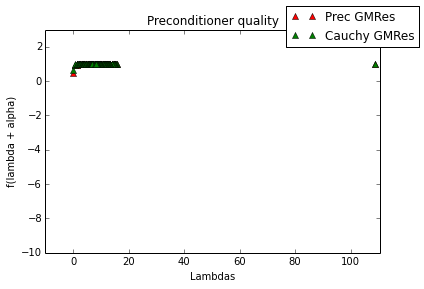
\includegraphics[scale=0.5]{images/producto.png}\\
Se puede ver que el producto se acerca al valor 1, por lo que la aproximación es valida. Cabe destacar que si la función es $f(x) = \frac{c}{x}$, al aplicar el producto, este tenderá a la constante c.

\subsubsection*{Análisis de iteraciones:}
Un factor importante pero no determinante es comprobar la cantidad de iteraciones que realiza el algoritmo. Se compararán los métodos de GMRes clásico, GMRes con precondicionador sin Cauchy y GMRes utilizando integral de contorno. Es importante mencionar que los últimos 2 resuelven sistemas de ecuaciones dentro de la ejecución de GMRes, por lo tanto poseen el metodo anidado.
Los parametros a variar serán la tolerancia del GMRes (Tol) principal para todos los casos, y para la integral de Cauchy, la tolerancia auxiliar (Aux\_tol) del GMRes utilizado dentro de la integral y el número de puntos (N) para la integración.

\begin{figure}[ht]
    \centering
    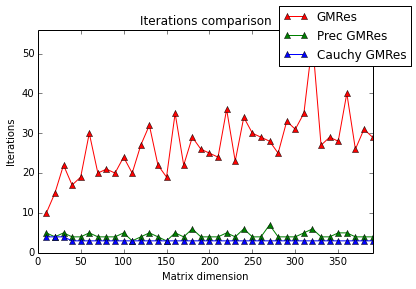
\includegraphics[scale=0.4]{images/i1.png}
    \caption{Tol: $10^{-6}$, Aux\_tol: $10^{-6}$, N: 128}
    \label{fig:1}
\end{figure}

\begin{figure}[ht]
    \centering
    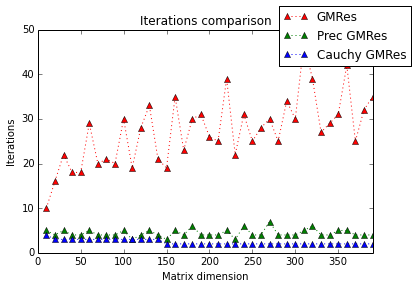
\includegraphics[scale=0.4]{images/i2.png}
    \caption{Tol: $10^{-6}$, Aux\_tol: $10^{-12}$, N: 32   }
    \label{fig:2}
\end{figure}
\newpage
\begin{figure}[ht]
    \centering
    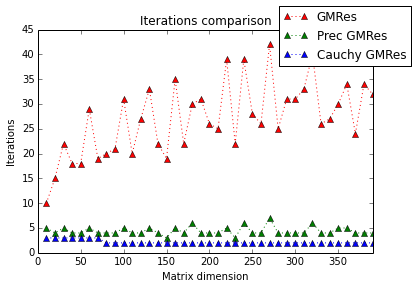
\includegraphics[scale=0.4]{images/i3.png}
    \caption{Tol: $10^{-6}$, Aux\_tol: $10^{-12}$, N: 16}
    \label{fig:3}
\end{figure}

\begin{figure}[ht]
    \centering
    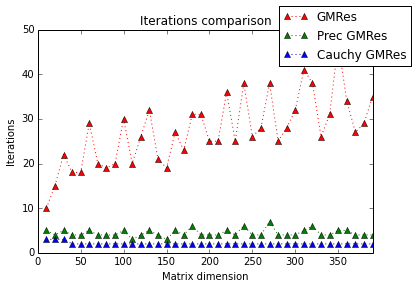
\includegraphics[scale=0.4]{images/i4.png}
    \caption{Tol: $10^{-6}$, Aux\_tol: $10^{-12}$, N: 8}
    \label{fig:4}
\end{figure}
\newpage
\begin{figure}[ht]
    \centering
    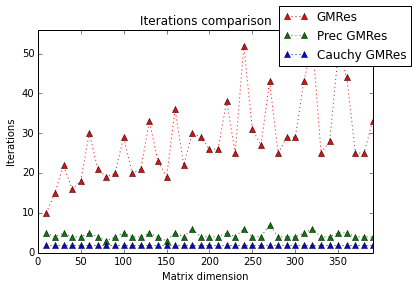
\includegraphics[scale=0.4]{images/i5.png}
    \caption{Tol: $10^{-6}$, Aux\_tol: $10^{-12}$, N: 4}
    \label{fig:5}
\end{figure}

\begin{figure}[ht]
    \centering
    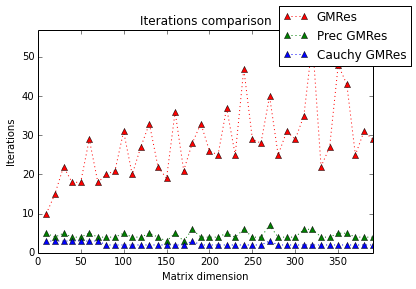
\includegraphics[scale=0.4]{images/i6.png}
    \caption{Tol: $10^{-6}$, Aux\_tol: $10^{-6}$, N: 16}
    \label{fig:6}
\end{figure}

Se puede ver que el número de iteraciones se mantiene independiente de la tolerancia y el número de puntos utilizados, donde se ven mejoras al aplicar los diferentes precondicionadores, pasando incluso desde las 40 iteraciones en GMRes clásico a menos de 5 para el uso de la formula de Cauchy.

\subsubsection*{Análisis de Backward Error}
Para los mismos casos se analiza como cambian los \emph{backward errors} para cada uno de estos.
Se utiliza al igual que el paso anterior, matrices de distinta dimensión, variando desde $10x10$, hasta $390x390$, de 10 en 10.\\
El backward error se define de la siguiente forma:
\begin{align}
    Error =  \frac{\|A\vec{x}-\vec{b}\|}{\|\vec{b}\|}
\end{align}

\begin{figure}[ht]
    \centering
    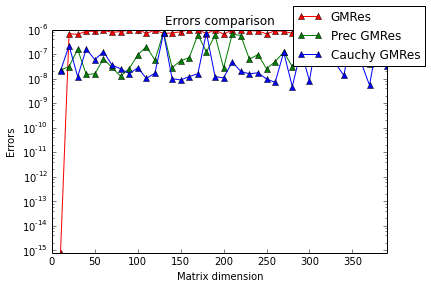
\includegraphics[scale=0.4]{images/b1.png}
    \caption{Tol: $10^{-6}$, Aux\_tol: $10^{-6}$, N: 128}
    \label{fig:7}
\end{figure}

\begin{figure}[ht]
    \centering
    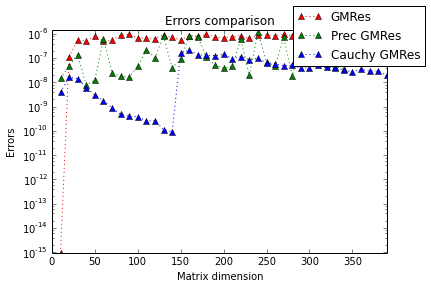
\includegraphics[scale=0.4]{images/b2.png}
    \caption{Tol: $10^{-6}$, Aux\_tol: $10^{-12}$, N: 32   }
    \label{fig:8}
\end{figure}
\newpage
\begin{figure}[ht]
    \centering
    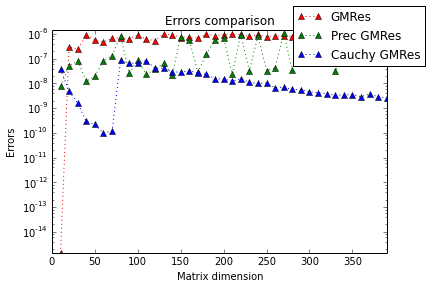
\includegraphics[scale=0.4]{images/b3.png}
    \caption{Tol: $10^{-6}$, Aux\_tol: $10^{-12}$, N: 16}
    \label{fig:9}
\end{figure}

\begin{figure}[ht]
    \centering
    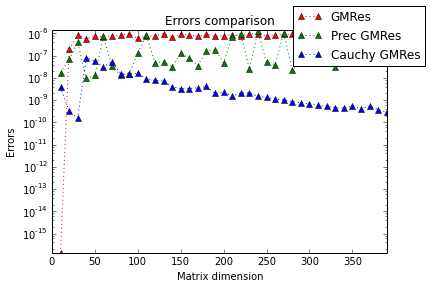
\includegraphics[scale=0.4]{images/b4.png}
    \caption{Tol: $10^{-6}$, Aux\_tol: $10^{-12}$, N: 8}
    \label{fig:10}
\end{figure}
\newpage
\begin{figure}[ht]
    \centering
    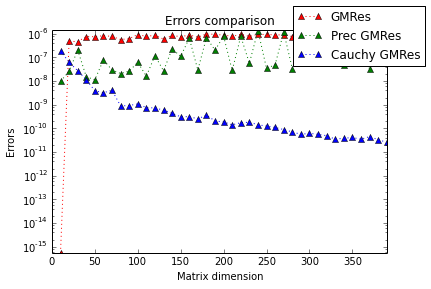
\includegraphics[scale=0.4]{images/b5.png}
    \caption{Tol: $10^{-6}$, Aux\_tol: $10^{-12}$, N: 4}
    \label{fig:11}
\end{figure}

\begin{figure}[ht]
    \centering
    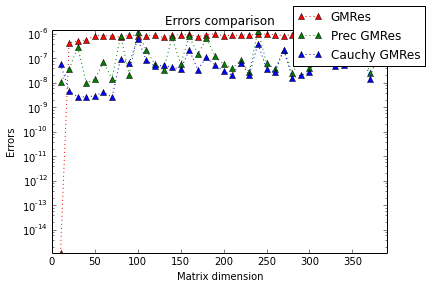
\includegraphics[scale=0.4]{images/b6.png}
    \caption{Tol: $10^{-6}$, Aux\_tol: $10^{-6}$, N: 16}
    \label{fig:12}
\end{figure}

A partir de este análisis, se puede obtener la primera conclusión importante, dado que el número de puntos afecta el error en la resolución del sistema, sin embargo, esto solo se nota cuando la tolerancia auxiliar, posee un valor menor. Se puede ver en la Figura 12, que para pocos puntos, pero una alta tolerancia, los errores se disparan y no se ve un patrón, por lo tanto se perturba.
Sin embargo podemos ver que los \emph{backwards errors} para la resolución son menores para los sistemas resueltos con el precondicionador calculado mediante Cauchy, comprobando en cierta parte la eficiencia de este método.

\subsubsection*{Análisis de Forward Error}
Para comprobar bien la eficiencia de los metodos desarrollados, también se analizarán los \emph{Forwards Errors}, con el objetivo de compararlo con la solución original, determinada manualmente para efectos de experimentación.\\
La definición del Forward Error es:
\begin{align}
    Error = \frac{\|\vec{x}-\vec{x}_{real}\|}{\|\vec{x}_{real}\|}
\end{align}

\begin{figure}[ht]
    \centering
    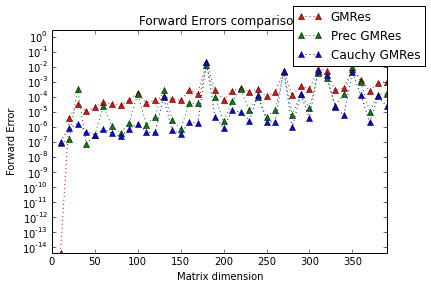
\includegraphics[scale=0.4]{images/x1.png}
    \caption{Tol: $10^{-6}$, Aux\_tol: $10^{-6}$, N: 128}
    \label{fig:13}
\end{figure}

\begin{figure}[ht]
    \centering
    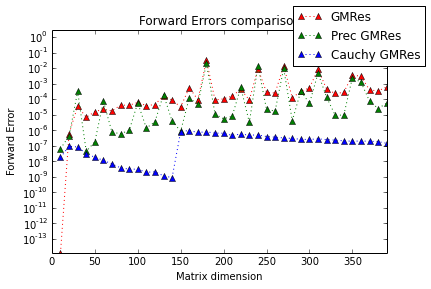
\includegraphics[scale=0.4]{images/x2.png}
    \caption{Tol: $10^{-6}$, Aux\_tol: $10^{-12}$, N: 32   }
    \label{fig:14}
\end{figure}
\newpage
\begin{figure}[ht]
    \centering
    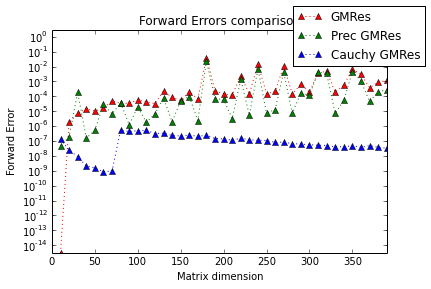
\includegraphics[scale=0.4]{images/x3.png}
    \caption{Tol: $10^{-6}$, Aux\_tol: $10^{-12}$, N: 16}
    \label{fig:15}
\end{figure}

\begin{figure}[ht]
    \centering
    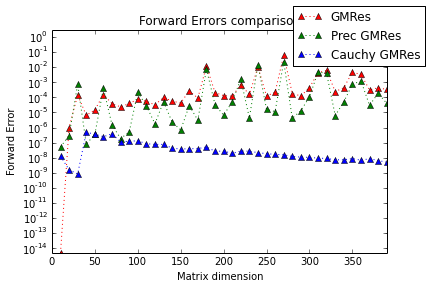
\includegraphics[scale=0.4]{images/x4.png}
    \caption{Tol: $10^{-6}$, Aux\_tol: $10^{-12}$, N: 8}
    \label{fig:16}
\end{figure}
\newpage
\begin{figure}[ht]
    \centering
    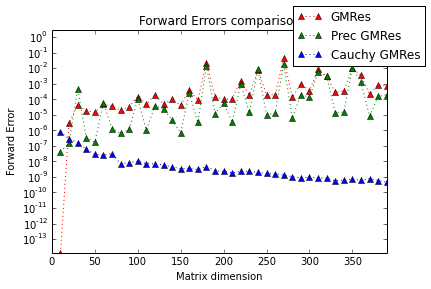
\includegraphics[scale=0.4]{images/x5.png}
    \caption{Tol: $10^{-6}$, Aux\_tol: $10^{-12}$, N: 4}
    \label{fig:17}
\end{figure}

\begin{figure}[ht]
    \centering
    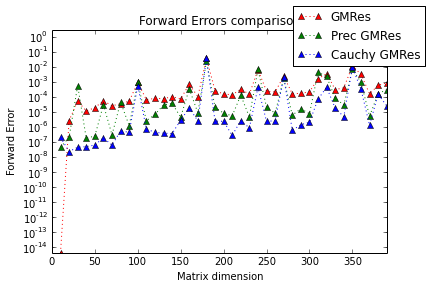
\includegraphics[scale=0.4]{images/x6.png}
    \caption{Tol: $10^{-6}$, Aux\_tol: $10^{-6}$, N: 16}
    \label{fig:18}
\end{figure}

Nuevamente se ve que debe existir un equilibrio entre la tolerancia auxiliar y el número de puntos. Se realizará un análisis en conjunto junto a los gráficos de tiempo a continuación. Por otro lado se observa que los errores respecto a la solución real con Cauchy son mucho mas bajos que los generados mediante los otros métodos. Con esto ya se prueba que si hablamos de calidad de la solución es recomendable utilizar precondicionador de Cauchy, sobre los otros métodos.
\newpage
\subsubsection*{Análisis de tiempos}
Mediante este análisis se pretende ver como afectan las variables de tolerancia y cantidad de puntos al tiempo de ejecución del algoritmo.

\begin{figure}[ht]
    \centering
    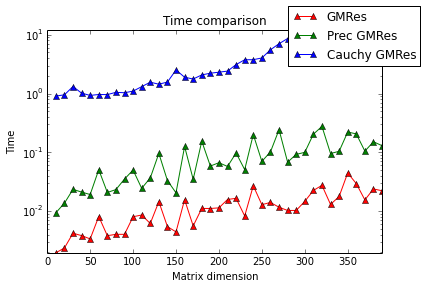
\includegraphics[scale=0.4]{images/t1.png}
    \caption{Tol: $10^{-6}$, Aux\_tol: $10^{-6}$, N: 128}
    \label{fig:19}
\end{figure}

\begin{figure}[ht]
    \centering
    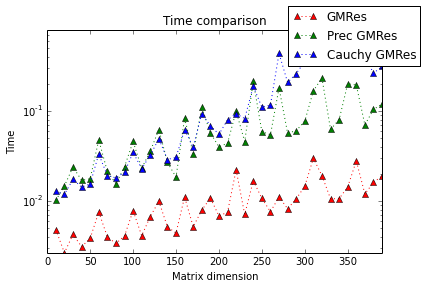
\includegraphics[scale=0.4]{images/t2.png}
    \caption{Tol: $10^{-6}$, Aux\_tol: $10^{-6}$, N: 4}
    \label{fig:20}
\end{figure}
\newpage
\begin{figure}[ht]
    \centering
    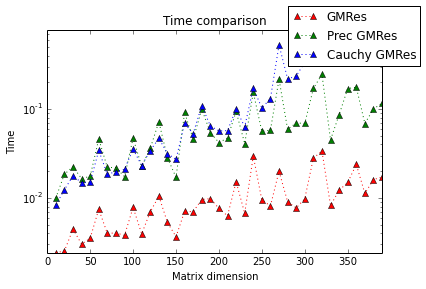
\includegraphics[scale=0.4]{images/t3.png}
    \caption{Tol: $10^{-6}$, Aux\_tol: $10^{-6}$, N: 4}
    \label{fig:21}
\end{figure}
\begin{figure}[ht]
    \centering
    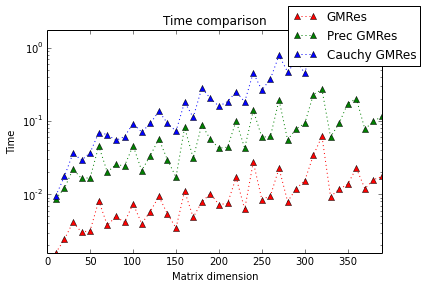
\includegraphics[scale=0.4]{images/t4.png}
    \caption{Tol: $10^{-6}$, Aux\_tol: $10^{-12}$, N: 4}
    \label{fig:22}
\end{figure}

En este análisis se puede ver, que existen pocas variaciones en los tiempos al varias la tolerancia. En cambio, para la variación de puntos de integración se observan cambios de hasta 3 ordenes de magnitud. Analizando esto junto con los gráficos de errores, se concluye que es conveniente usar pocos puntos y una alta tolerancia, dado que la tolerancia auxiliar no afectará demasiado el tiempo de ejecución, la baja cantidad de puntos hará incluso el algoritmo más rápido, y como se ha visto en los gráficos, con esta combinación de parámetros, la solución posee unos resultados pequeños, dado que se ve que la tolerancia auxiliar es el parámetro que mas afecta en la calidad de la solución

\subsubsection*{Análisis Tiempo v/s Precisión}
El último análisis muestra el gráfico de Tiempos de ejecución para diferentes niveles de precisión. Lamentablemente, por un problema de desconfiguración del gráfico en matplotlib, el gráfico logarítmico no se muestra bien. 


\begin{figure}[ht]
    \centering
    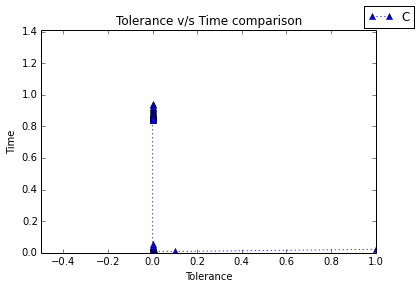
\includegraphics[scale=0.4]{images/p.png}
    \caption{Tol: $10^{-6}$, N: 4}
    \label{fig:23}
\end{figure}

A pesar de la mala visión que provee el gráfico, se ve que al disminuir la precisión el tiempo va aumentando, sin embargo, las variaciones no pasan de 1 segundo, para variaciones de 50 ordenes de mágnitud. Con esto se comprueba que lo que más afecta el tiempo de computo son los puntos de la integral.\newpage


\subsection{Conclusión}
Como conclusiones generales, se puede decir que el uso de un precondicionador efectivamente, mejora la calidad de la solución y los tiempos de ejecución para matrices positivas definidas y mal condicionadas. Se ve mediante la experimentación que el utilizar la integral de Cauchy es muchísimo mas conveniente en cuanto a calidad que los otros métodos vistos. Mientras que por el lado del tiempo, este algoritmo tiene un alto nivel de paralelización, debido a la cantidad de GMRes que podrían calcularse de forma paralela. Aún así, para esto, se debe analizar los tiempos de envío de información, y con estos datos, realizar el estudio real de los tiempos de ejecución, entre versiones paralela y secuencial. Sin embargo, se toma como supuesto que debiera ser mas rápido que la versión secuencial. En pocas palabras, mientras la matriz cumpla las condiciones iniciales, y se prefiera calidad sobre tiempo, es altamente recomendable utilizar precondicionador con fórmula de Cauchy.


\bibliographystyle{plain}
\bibliography{Referencias}

\end{document}
